\documentclass[preprint,12pt]{elsarticle}

\usepackage{amsmath,amssymb,amsthm,booktabs,graphicx,microtype,url,xspace,float,tabularx}
\usepackage[ruled,vlined,linesnumbered]{algorithm2e}
\usepackage{tikz}
\usetikzlibrary{arrows.meta,positioning,calc,fit}
\graphicspath{{figures/}}

\journal{Theoretical Computer Science}

\newcommand{\vol}{\operatorname{vol}}
\newcommand{\HT}{H^{T}}
\newcommand{\NEST}{\textsc{Nest}\xspace}
\newcommand{\GNEST}{\textsc{Nest-G}\xspace}
\newcommand{\lca}{\operatorname{lca}}
\newtheorem{theorem}{Theorem}
\newtheorem{proposition}[theorem]{Proposition}
\newtheorem{lemma}[theorem]{Lemma}
\newtheorem{corollary}[theorem]{Corollary}
\theoremstyle{definition}
\newtheorem{definition}[theorem]{Definition}
\newtheorem{problem}[theorem]{Problem}

\newcommand{\NESTGainVsHCSE}{0.5468}
\newcommand{\NESTGainVsHCSECI}{0.0218}
\newcommand{\NESTGainVsBBM}{0.5213}
\newcommand{\NESTGainVsBBMCI}{0.0101}
\newcommand{\NESTGainVsBestExternal}{0.4239}
\newcommand{\NESTGainVsBestExternalCI}{0.0086}
\newcommand{\OursWins}{500/500}
\newcommand{\OursWithinOne}{500/500}
\newcommand{\AuditOneRate}{69\%}
\newcommand{\AuditCompoundRate}{50\%}
\newcommand{\RealWins}{4/4}
\newcommand{\FairNESTExact}{249/250}
\newcommand{\FairHCSEExact}{2/250}
\newcommand{\FairBBMExact}{1/250}
\newcommand{\FairNESTMeanGap}{0.00032\%}
\newcommand{\FairNESTWorstGap}{0.07990\%}
\newcommand{\ScaleNFourteenExact}{99/100}
\newcommand{\ScaleNSixteenExact}{22/25}
\newcommand{\ScaleCombinedExact}{370/375}

\emergencystretch=3em
\widowpenalty=10000
\clubpenalty=10000
\displaywidowpenalty=10000

\begin{document}

\begin{frontmatter}
\title{Complexity and Certified Tree-Rearrangement Search for
Structural-Entropy Hierarchies}

% HUMAN METADATA GATE: replace with the approved author list, affiliations,
% ORCIDs, and corresponding-author details before journal upload.
\author{Anonymous Authors}
\address{Affiliation withheld for review}

\begin{abstract}
Structural entropy scores a graph hierarchy by the description length induced
by its encoding tree. Existing constructors return low-entropy trees, but two
basic questions remain: which restricted optimization problem is already
computationally hard, and how can a constructed tree be improved beyond local
rotations without sacrificing exact scoring? We prove that balanced
two-module structural-entropy minimization is NP-hard on simple unweighted
cubic graphs through an exact affine equivalence with Minimum Bisection. We
then derive exact entropy changes for rooted nearest-neighbor interchange
(NNI) and subtree prune-and-regraft. The graft change has equivalent edge--LCA
and changed-incidence forms; these identities show that NNI is a restricted
graft and yield checkable certificates for the declared neighborhoods. They
lead to \GNEST, which alternates exact NNI descent with exhaustive
best-improvement grafting and fully rescores every accepted endpoint. Two
independent graft evaluators agree with full entropy recomputation on 1,680
legal weighted-tree moves to within $1.5\times10^{-15}$ bits. On five exact
diagnostic instances where rotation-only search stopped above the optimum,
grafting reaches the optimum in every case. Together, the complexity result,
edit calculus, and certified search connect the global combinatorial obstacle
to an auditable optimization procedure in encoding-tree space.
\end{abstract}


\begin{keyword}
structural entropy \sep hierarchical clustering \sep tree search \sep
nearest-neighbor interchange \sep subtree grafting \sep graph bisection
\end{keyword}
\end{frontmatter}

\section{Introduction}\label{sec:introduction}

Many networks have meaningful organization at several resolutions. Vertices
form local groups, related groups form larger modules, and the desired output
is therefore a hierarchy rather than a flat partition. Structural entropy
expresses this organization as the description length of an encoding
tree~\cite{li2016}. The objective has motivated hierarchy construction in
graph clustering~\cite{pan2025}, chromatin-domain detection
~\cite{zhang2021supertad}, and a growing range of graph-learning
applications~\cite{su2025survey}.

Optimizing the tree objective raises two different questions. The first is
global: which restricted forms of structural-entropy minimization already
contain a hard combinatorial problem? The second is geometric: once a tree has
been constructed, which topology edits can expose an improvement and which
certificate is obtained when search terminates? These questions are linked by
the objective but require different tools. A complexity reduction identifies
the hard partitioning core; an edit identity explains the local search space.

A preliminary conference manuscript addressed the second question with
rooted nearest-neighbor interchange (NNI). Its method, \NEST, derived an exact
NNI entropy change, refined several initial trees, crossed selected two-move
barriers, and compared the returned trees with exact optima on small graphs.
NNI modifies one internal edge and is consequently inexpensive and easy to
certify. Its locality is also a limitation: moving a subtree across several
levels may require a sequence of rotations whose intermediate trees increase
the objective and are rejected by monotone descent.

This article develops both questions beyond rotation-only search. For
complexity, we isolate balanced two-module structural entropy and prove an
exact equivalence with Minimum Bisection on regular graphs. For tree search,
we add subtree prune-and-regraft, which relocates an entire subtree in one
operation. The edge--LCA expansion gives an exact graft change, while a second
derivation cancels every unchanged cluster--parent incidence. The two formulas
support independent implementation checks and identify precisely where a
graft can alter the objective.

Our contributions are as follows.
\begin{itemize}
  \item We prove that the decision and optimization forms of balanced
  two-module structural entropy are NP-hard on simple unweighted cubic graphs
  through the identity
  $H^{\mathcal P}(G)=\log_2(n/2)+c(\mathcal P)/|E|$.
  \item We give exact formulas for weighted NNI and rooted subtree grafting,
  including a path-supported cancellation theorem and the inclusion of the
  NNI neighborhood in the graft neighborhood.
  \item We introduce \GNEST, an exact best-improvement NNI--graft refiner.
  Exhaustive termination returns a checkable certificate for the declared
  graft neighborhood and, by inclusion, for the NNI neighborhood.
  \item We validate two independent graft-delta calculations against full
  recomputation on 1,680 moves and show, in a diagnostic exact audit, that
  graft search repairs all five residual failures of rotation-only \NEST.
  \item We retain the preliminary study's frozen 500-graph constructor study
  and 375-graph exact audit as the reference rotation-only evaluation, thereby
  separating inherited evidence from the new graft experiments.
\end{itemize}

The remainder of the article defines the problem family
(Section~\ref{sec:preliminaries}), proves the constrained hardness result
(Section~\ref{sec:hardness}), develops the edit calculus
(Section~\ref{sec:calculus}), gives the certified algorithm
(Section~\ref{sec:algorithm}), and reports reproducible audits
(Section~\ref{sec:experiments}).

\section{Structural entropy and problem variants}\label{sec:preliminaries}

Let $G=(V,E,w)$ be an undirected graph with nonnegative edge weights. Write
$d_u=\sum_v w_{uv}$, $M=\vol(V)=\sum_u d_u$, and
$W(A,B)=\sum_{u\in A,v\in B}w_{uv}$ for disjoint vertex sets. For
$S\subseteq V$, let $V_S=\sum_{u\in S}d_u$ and let $g_S$ be the weight of
edges with exactly one endpoint in $S$.

An encoding tree $T$ has one leaf for every vertex. Each tree node $a$
represents the cluster $S_a$ of descendant leaves, and $a^{-}$ denotes its
parent. The structural entropy of $G$ under $T$ is
\begin{equation}
 H^T(G)=-\sum_{a\neq r}\frac{g_{S_a}}{M}
 \log_2\frac{V_{S_a}}{V_{S_{a^-}}}.
 \label{eq:tree-se-journal}
\end{equation}
Lower values indicate shorter graph-dependent descriptions. Zero-volume
components contribute zero and may be attached after optimizing the
positive-volume part, so the theory below assumes positive volume whenever a
logarithm is evaluated.

Two equivalent views will be useful. The node view is
Eq.~\eqref{eq:tree-se-journal}. In the edge view, every edge is charged at the
least common ancestor of its endpoints:
\begin{equation}
 H^T(G)=\sum_{uv\in E}\frac{w_{uv}}{M}
 \log_2\frac{V_{\lca_T(u,v)}^2}{d_ud_v}.
 \label{eq:edge-lca-journal}
\end{equation}
The equivalence follows by expanding each cut term and telescoping the code
lengths along the two leaf-to-LCA paths.

We distinguish three optimization problems.
\begin{problem}[Tree structural entropy]
Given $G$, find an encoding tree minimizing Eq.~\eqref{eq:tree-se-journal}.
\end{problem}

\begin{problem}[Two-dimensional structural entropy]
Given $G$, find a height-two encoding tree, equivalently a nonempty partition
$\mathcal P=\{S_1,\ldots,S_K\}$, minimizing structural entropy.
\end{problem}

\begin{problem}[Balanced two-module structural entropy]
Given a regular graph of even order, minimize two-dimensional structural
entropy over partitions $\{S,V\setminus S\}$ satisfying $|S|=|V|/2$.
\end{problem}

The third problem is a restriction of the second. We state it separately
because its balance constraint is essential to the reduction in
Section~\ref{sec:hardness}.

For search, we work with rooted binary trees. Prior work establishes that every
encoding tree admits a binary refinement of no greater structural entropy
\cite{zhang2021supertad,pan2025}. Thus a global optimum exists in the binary
class, although constructors may initially return multiway trees and refine
them before search.

\section{A hard balanced partitioning core}\label{sec:hardness}

This section isolates a constrained form of structural entropy that is already
computationally hard. The result also explains why cut quality alone does not
characterize a general two-dimensional optimum: module volumes enter the
objective unless they are controlled.

We use the following decision form. An instance consists of a simple cubic
graph $G=(V,E)$ with even $n=|V|$ and an integer $b$. The question is whether
there exists $S\subset V$ with $|S|=n/2$ such that the height-two tree induced
by $\{S,V\setminus S\}$ has entropy at most
$\log_2(n/2)+b/|E|$. The threshold is represented by the integer pair
$(n,b)$; no numerical approximation to the logarithm is part of the input.

For a partition $\mathcal P=\{S_1,\ldots,S_K\}$, let $e_i$ be the internal
edge weight of $S_i$. Directly expanding Eq.~\eqref{eq:tree-se-journal} gives
\begin{align}
 H^{\mathcal P}(G)
 &= -\frac{1}{M}\sum_{u\in V}d_u\log_2\frac{d_u}{V_{S(u)}}
    -\frac{1}{M}\sum_{i=1}^{K}g_i\log_2\frac{V_i}{M}\notag\\
 &= C_G+\frac{1}{M}\sum_{i=1}^{K}
 \left[2e_i\log_2 V_i+g_i\log_2 M\right],
 \label{eq:partition-form}
\end{align}
where $C_G=-M^{-1}\sum_ud_u\log_2d_u$ does not depend on the partition and
$V_i-g_i=2e_i$.

\begin{lemma}[Balanced regular identity]\label{lem:bisection-identity}
Let $G$ be a loop-free $d$-regular graph with even order $n$ and
$m=|E|=dn/2$. For a balanced bipartition $\mathcal P$ with cut size
$c(\mathcal P)$,
\begin{equation}
 H^{\mathcal P}(G)=\log_2\frac{n}{2}+\frac{c(\mathcal P)}{m}.
 \label{eq:balanced-identity}
\end{equation}
Consequently, for two balanced bipartitions $\mathcal P$ and $\mathcal Q$,
$H^{\mathcal P}(G)-H^{\mathcal Q}(G)=
[c(\mathcal P)-c(\mathcal Q)]/m$.
\end{lemma}

\begin{proof}
Every vertex has degree $d$, both modules have volume $dn/2=M/2$, and both
module cuts equal $c(\mathcal P)$. The leaf contribution to the height-two
tree is
\[
 -\frac{1}{M}\sum_{u\in V}d\log_2\frac{d}{M/2}
 =\log_2(n/2).
\]
The two module contributions sum to
$-2c(\mathcal P)M^{-1}\log_2(1/2)=c(\mathcal P)/m$.
Adding the terms proves Eq.~\eqref{eq:balanced-identity}.
\end{proof}

\begin{theorem}[Constrained structural-entropy hardness]
\label{thm:balanced-hardness}
The decision form of balanced two-module structural entropy is NP-complete on
simple unweighted cubic graphs. Consequently, computing an optimal balanced
two-module encoding tree is NP-hard on the same class.
\end{theorem}

\begin{proof}
Minimum Bisection is NP-complete on simple cubic graphs
\cite{bui1987graph}. Map an instance $(G,b)$ identically to the entropy
decision instance $(G,b)$. The mapping is polynomial and introduces neither
weights nor auxiliary vertices. By Lemma~\ref{lem:bisection-identity}, a
balanced partition $\mathcal P$ satisfies
$H^{\mathcal P}(G)\leq\log_2(n/2)+b/m$ if and only if
$c(\mathcal P)\leq b$. This proves NP-hardness. A balanced set $S$ is a
polynomial certificate, and the equivalent integer comparison
$c(\mathcal P)\leq b$ verifies it in polynomial time; hence the decision
problem is in NP. An optimizer would decide the problem by comparing its
returned cut size with $b$, so the optimization form is NP-hard.
\end{proof}

The balance constraint cannot simply be discarded. On the 10-vertex
pentagonal prism and M\"obius ladder, exhaustive enumeration finds a $4/6$
partition with entropy $2.625497$ bits, below the best balanced value
$2.655261$. Thus regularity and exactly two nonempty modules do not force a
bisection. This counterexample delineates the theorem's scope and rules out an
otherwise tempting transfer to unconstrained two-module optimization.

\section{Exact calculus for local and nonlocal tree edits}
\label{sec:calculus}

\subsection{Rooted nearest-neighbor interchange}

Consider three disjoint subtrees $A,B,C$ inside a local cluster
$P=A\cup B\cup C$. A rooted NNI replaces $((A,B),C)$ by
$(A,(B,C))$. Let $X=A\cup B$ and $Y=B\cup C$.

\begin{proposition}[Exact weighted NNI delta]\label{prop:nni-delta-journal}
For $V_X,V_Y,V_P>0$, the entropy change is
\begin{equation}
 \Delta_{\mathrm{NNI}} H^T=
 \frac{2}{M}\left[
 W(A,B)\log_2\frac{V_P}{V_X}+
 W(B,C)\log_2\frac{V_Y}{V_P}
 \right].
 \label{eq:nni-delta-journal}
\end{equation}
The other rooted alternative follows by exchanging $A$ and $B$.
\end{proposition}

\begin{proof}
Only the code lengths involving $A,B,C,X$, and $Y$ change. Substitute
$g_X=g_A+g_B-2W(A,B)$ and
$g_Y=g_B+g_C-2W(B,C)$ into
Eq.~\eqref{eq:tree-se-journal}. The coefficients of $g_A,g_B,g_C$ telescope,
leaving Eq.~\eqref{eq:nni-delta-journal}.
\end{proof}

The identity permits exhaustive best-improvement descent: enumerate every
eligible internal edge, commit the most negative exact delta, and stop when no
delta is negative. Termination certifies one-NNI local optimality for the
returned tree.

\subsection{Rooted subtree prune-and-regraft}

A legal graft chooses a non-root source subtree $S$ and a target subtree $Q$
that is neither an ancestor nor a descendant of $S$. It detaches $S$,
suppresses the resulting unary parent, and replaces $Q$ by a new binary parent
with children $S$ and $Q$. Same-parent choices are omitted because they
recreate the same unordered hierarchy. Figure~\ref{fig:graft} contrasts the
short-range and long-range edits.

\begin{figure}[t]
\centering
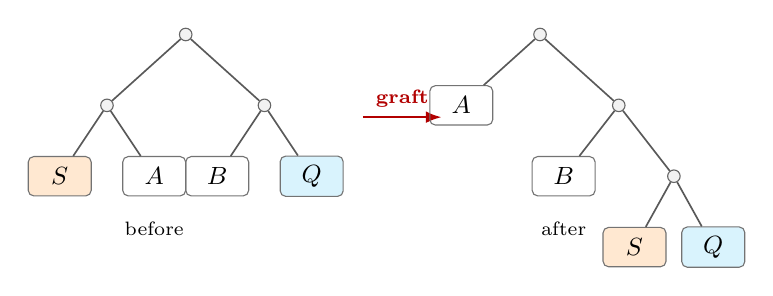
\begin{tikzpicture}[
  node distance=5mm and 9mm,
  every node/.style={font=\small},
  internal/.style={circle,draw=black!60,fill=black!5,inner sep=1.6pt},
  block/.style={rounded corners=2pt,draw=black!55,minimum width=8mm,
                minimum height=5mm},
  link/.style={draw=black!65,line width=.6pt}
]
\node[internal] (r1) at (0,0) {};
\node[internal] (u1) at (-1,-.9) {};
\node[internal] (v1) at (1,-.9) {};
\node[block,fill=orange!18] (s1) at (-1.6,-1.8) {$S$};
\node[block] (a1) at (-.4,-1.8) {$A$};
\node[block] (b1) at (.4,-1.8) {$B$};
\node[block,fill=cyan!15] (q1) at (1.6,-1.8) {$Q$};
\draw[link] (r1)--(u1) (r1)--(v1) (u1)--(s1) (u1)--(a1)
            (v1)--(b1) (v1)--(q1);
\node[font=\scriptsize,below=2mm of a1] {before};

\draw[-{Latex[length=2mm]},red!70!black,line width=.8pt]
  (2.25,-1.05)--(3.25,-1.05);
\node[font=\scriptsize\bfseries,text=red!70!black] at (2.75,-.82) {graft};

\node[internal] (r2) at (4.5,0) {};
\node[block] (a2) at (3.5,-.9) {$A$};
\node[internal] (v2) at (5.5,-.9) {};
\node[block] (b2) at (4.8,-1.8) {$B$};
\node[internal] (z2) at (6.2,-1.8) {};
\node[block,fill=orange!18] (s2) at (5.7,-2.7) {$S$};
\node[block,fill=cyan!15] (q2) at (6.7,-2.7) {$Q$};
\draw[link] (r2)--(a2) (r2)--(v2) (v2)--(b2) (v2)--(z2)
            (z2)--(s2) (z2)--(q2);
\node[font=\scriptsize,below=2mm of b2] {after};
\end{tikzpicture}
\caption{A graft detaches the source subtree $S$ and inserts it next to target
$Q$, suppressing the old unary parent. Unlike one NNI, the source and target
may be separated by several tree levels.}
\label{fig:graft}
\end{figure}

\begin{theorem}[Exact edge--LCA graft delta]\label{thm:graft-lca}
Let $T'$ be obtained from $T$ by a legal graft. Then
\begin{equation}
 H^{T'}(G)-H^T(G)=\frac{2}{M}\sum_{uv\in E}w_{uv}
 \log_2\frac{V_{\lca_{T'}(u,v)}}{V_{\lca_T(u,v)}}.
 \label{eq:graft-lca-delta}
\end{equation}
Every edge whose LCA cluster and LCA volume are unchanged contributes zero.
\end{theorem}

\begin{proof}
Apply Eq.~\eqref{eq:edge-lca-journal} to $T'$ and $T$. The factors $d_ud_v$
depend only on the graph and cancel. Combining the two logarithms yields
Eq.~\eqref{eq:graft-lca-delta}.
\end{proof}

The all-edge sum is a correctness-oriented formula. A second exact form makes
the locality explicit. Let $\mathcal C(T)$ be the non-root clusters of $T$ and
$p_T(C)$ the parent cluster of $C$. Define
\[
 \psi(C,P)=-\frac{g_C}{M}\log_2\frac{V_C}{V_P}.
\]
Let $I(T)=\{(C,p_T(C)):C\in\mathcal C(T)\}$ be the set of non-root
cluster--parent incidences. For a graft from $T$ to $T'$, define
$\mathcal A_-=I(T)\setminus I(T')$ and
$\mathcal A_+=I(T')\setminus I(T)$.

\begin{theorem}[Changed-incidence graft formula]\label{thm:graft-path}
For a legal graft from $T$ to $T'$ ,
\begin{equation}
 H^{T'}(G)-H^T(G)=
 \sum_{(C,P)\in\mathcal A_+}\psi(C,P)
 -\sum_{(C,P)\in\mathcal A_-}\psi(C,P).
 \label{eq:graft-path-delta}
\end{equation}
Every incidence in $\mathcal A_-\cup\mathcal A_+$ lies on the source-removal
path, the target-insertion path, or at the new parent of $S$ and $Q$.
\end{theorem}

\begin{proof}
Write Eq.~\eqref{eq:tree-se-journal} as the sum of $\psi(C,p_T(C))$ over
$C\in\mathcal C(T)$. Detaching $S$ changes only ancestors between the old
parent of $S$ and the first common ancestor of the source and target paths;
inserting $S$ changes only the corresponding target ancestors and creates the
parent $S\cup Q$. Every cluster and parent outside these paths has the same
leaf set before and after the edit, so its incidence belongs to
$I(T)\cap I(T')$ and cancels. The noncancelling old and new terms are exactly
$\mathcal A_-$ and $\mathcal A_+$, which proves both the identity and the path
support statement.
\end{proof}

The theorem is stronger than a cut-edge-only shortcut. When $S$ is inserted,
ancestor clusters on the target path gain its volume; when $S$ is removed,
clusters on the source path lose it. Therefore an edge with neither endpoint
in $S$ can still change contribution when its LCA lies on an affected path.

\subsection{Relation between the neighborhoods}

\begin{proposition}[NNI is a restricted graft]\label{prop:nni-is-graft}
Every rooted NNI neighbor of a binary tree is also a legal rooted graft
neighbor.
\end{proposition}

\begin{proof}
For $((A,B),C)\rightarrow(A,(B,C))$, detach $C$ and graft it next to $B$.
Suppressing the old parent exposes $(A,B)$, and inserting the new parent of
$B,C$ produces $(A,(B,C))$. Grafting $C$ next to $A$ gives the symmetric NNI
alternative.
\end{proof}

\begin{corollary}\label{cor:graft-cert}
A tree with no improving legal graft has no improving rooted NNI.
\end{corollary}

The converse fails on the audited instances in Section~\ref{sec:graft-audit}:
trees certified against one-step NNI admit an improving graft. Grafting thus
tests a strictly richer neighborhood on those instances rather than merely
rescoring the same rotations.

\begin{table}[H]
\centering
\small
\caption{Relation between the two exact edit neighborhoods. Tree distance is
the maximum source relocation accomplished by one move. A certificate means
that all legal candidates in the stated neighborhood have nonnegative exact
entropy change.}
\label{tab:neighborhoods}
\begin{tabularx}{\textwidth}{@{}lccX@{}}
\toprule
Edit & Candidates & Range & Exhaustive stopping certificate \\
\midrule
Rooted NNI & $O(n)$ & one edge & one-NNI local optimum \\
Rooted graft & $O(n^2)$ & any legal path & graft-local optimum (and therefore one-NNI local) \\
\bottomrule
\end{tabularx}
\end{table}

\section{Certified NNI--graft search}\label{sec:algorithm}

\GNEST separates tree construction from topology refinement. It accepts any
rooted binary initializer, performs exact NNI descent, searches the complete
legal graft neighborhood, and reruns NNI descent after each accepted graft.
Every committed endpoint is independently rescored with
Eq.~\eqref{eq:tree-se-journal}.

\begin{algorithm}[t]
\caption{Exact certified NNI--graft refinement}\label{alg:graft-nest}
\KwIn{Graph $G$, binary tree $T$, tolerance $\varepsilon$}
fully rescore $T$ and set $h\leftarrow H^T(G)$\;
\Repeat{no accepted graft exists}{
  repeatedly commit the most negative exact NNI delta until none is below
  $-\varepsilon$; fully verify every committed tree\;
  enumerate every legal ordered source--target graft of the current tree\;
  evaluate each candidate by Eq.~\eqref{eq:graft-lca-delta} or
  Eq.~\eqref{eq:graft-path-delta}\;
  \eIf{the best fully rescored graft endpoint is below $h-\varepsilon$}{
    commit it and update $h$\;
  }{
    \textbf{break}\;
  }
}
\Return{$T$, $h$, and the final neighborhood audit}
\end{algorithm}

\begin{proposition}[Monotonicity and termination]\label{prop:termination}
Algorithm~\ref{alg:graft-nest} monotonically decreases structural entropy and
terminates after finitely many accepted moves.
\end{proposition}

\begin{proof}
The algorithm commits a move only after its independently recomputed endpoint
is at least $\varepsilon$ below the current objective. The number of rooted
binary trees on a fixed labeled leaf set is finite, and strict decrease
prevents revisiting a tree.
\end{proof}

\begin{proposition}[Declared-neighborhood certificate]\label{prop:union-cert}
If Algorithm~\ref{alg:graft-nest} reaches its natural stopping condition, its
output has neither an improving rooted NNI nor an improving legal graft under
the stated tolerance.
\end{proposition}

\begin{proof}
The final NNI descent exhausts all rooted NNI candidates. The subsequent graft
sweep exhausts all legal ordered source--target pairs and finds none whose
verified endpoint improves the objective. Proposition~\ref{prop:nni-is-graft}
also implies the NNI part of the certificate from exhaustive graft locality,
but we retain the explicit NNI sweep because its closed-form candidates are
cheaper to evaluate.
\end{proof}

For $n$ leaves there are $O(n)$ rooted NNI candidates and $O(n^2)$ ordered
graft candidates per sweep. A correctness-first graft candidate is rebuilt
and rescored in $O(n+|E|)$ time, giving
$O(n^2(n+|E|))$ time for one exhaustive reference sweep. The independent
changed-incidence evaluator instead recomputes only terms whose
cluster--parent relation changes. Cached volumes, cuts, and LCA buckets can
replace both reference scans without changing the identities. Candidate
grafts are independent at a fixed tree, so a sweep can also be evaluated in
parallel. The present implementation uses the slower reference path so that
the certificate does not depend on an unvalidated cache.

For small graphs, the final endpoint is compared with an independent exact
subset dynamic program. For every nonempty $S\subseteq V$, let $F(S)$ be the
minimum contribution below a binary node representing $S$. Then
\begin{equation}
\begin{split}
F(\{v\})&=0,\\
F(S)&=\min_{A\mathbin{\dot\cup}B=S}\left\{F(A)+F(B)
-\frac{g_A}{M}\log_2\frac{V_A}{V_S}
-\frac{g_B}{M}\log_2\frac{V_B}{V_S}\right\}.
\end{split}
\label{eq:journal-dp}
\end{equation}
Enumerating unordered splits gives $O(3^n)$ time and $O(2^n)$ memory. Binary
sufficiency makes $F(V)$ a global structural-entropy optimum
\cite{zhang2021supertad,pan2025}.

\section{Computational verification and empirical audits}
\label{sec:experiments}

The evaluation is organized by claim dependency. We first check the algebraic
identity used in the reduction, then validate the new graft operator, next
examine the five known rotation-only misses, and finally summarize the frozen
broad and exact benchmarks inherited from the preliminary study. All
selections use structural entropy only; exact optima are consulted after
selection.

\subsection{Finite checks of the balanced identity}

An independent implementation enumerated 3,199 unordered balanced partitions
across 23 regular graphs drawn from cycles, complete graphs, complete
bipartite graphs, prisms, M\"obius ladders, and circulant families. The direct
two-dimensional entropy and Eq.~\eqref{eq:balanced-identity} agreed within
$1.34\times10^{-15}$ bits. Entropy minimizers and minimum bisections agreed on
every graph. A separate enumeration of 13,697 unrestricted bipartitions found
the two 10-vertex counterexamples reported in Section~\ref{sec:hardness}. The
finite check supports the algebra and guards against an invalid removal of the
balance constraint; Theorem~\ref{thm:balanced-hardness} is established by the
proof rather than by enumeration.

\subsection{Independent validation of graft deltas}\label{sec:graft-validation}

We generate 20 connected weighted graphs with five to nine vertices and one
random binary tree per graph. For every legal graft, we compare three values:
full recomputation of Eq.~\eqref{eq:tree-se-journal}, the edge--LCA delta in
Eq.~\eqref{eq:graft-lca-delta}, and the changed-incidence delta in
Eq.~\eqref{eq:graft-path-delta}. Across 1,680 legal moves, both delta evaluators
match full recomputation to floating-point precision; the largest absolute
discrepancy is below $1.5\times10^{-15}$ bits. Every candidate preserves a
rooted binary topology and exactly one copy of every leaf.

Four additional best-improvement runs check end-to-end behavior. Each accepted
graft strictly reduces the independently rescored objective, and exhaustive
enumeration at termination finds no improving legal graft among 88--124 final
candidates. These tests validate the reference implementation and the stated
neighborhood certificate separately from the method's optimization quality.

\subsection{Repairing the residual exact misses}\label{sec:graft-audit}

The earlier sealed exact audit contained five instances on which 32
coalescent starts followed by NNI and bounded two-step search missed the exact
dynamic-programming optimum. We reconstruct the same graphs and restart
streams, apply exhaustive best-improvement grafting to each returned tree, and
consult the exact optimum only after selecting the lowest-entropy endpoint.
Table~\ref{tab:graft-repair} reports the diagnostic result.

\begin{table}[t]
\centering
\small
\setlength{\tabcolsep}{4pt}
\caption{Diagnostic graft audit on all five known residual misses. ``Improved
starts'' counts the original 32 rotation-refined starts whose entropy is
further reduced by grafting. The final gap is measured against the independent
subset-DP optimum; lower is better.}
\label{tab:graft-repair}
\begin{tabular}{rllrrr}
\toprule
$n$ & Regime & Seed & NNI gap (bits) & Improved starts & Graft gap \\
\midrule
12 & Clean          & 168  & 0.001323 & 31/32 & 0 \\
14 & Weak hierarchy & 3004 & 0.002440 & 18/32 & 0 \\
16 & Noisy          & 4001 & 0.005274 & 23/32 & 0 \\
16 & Noisy          & 4002 & 0.007208 & 28/32 & 0 \\
16 & Weak hierarchy & 4002 & 0.010305 & 26/32 & 0 \\
\bottomrule
\end{tabular}
\end{table}

Grafting reaches the exact optimum on all five cases. It improves between 18
and 31 of the 32 starts per graph, showing that the outcome is not confined to
one fortuitous restart. These instances were selected precisely because
rotation-only search missed them; the result therefore demonstrates the
mechanism and a strict neighborhood advantage on the diagnosed cases. It is
not used to estimate the frequency of improvement on unseen graphs.

\subsection{Frozen rotation-only benchmark}

The preliminary study contains 100 graphs from each of five 64-vertex
hierarchical stochastic block-model regimes: clean, noisy, imbalanced,
weighted, and weak hierarchy. \NEST uses a fixed pool of SE agglomeration,
recursive SE, and Paris initial trees, refines each by exact NNI and bounded
two-move search, and returns the lowest independently rescored endpoint.
HCSE and BBM are external comparators and are not added to the initializer
pool. Table~\ref{tab:main-h} reproduces the frozen results.

\begin{table}[H]
\centering\small
\caption{Mean tree structural entropy $H^T$ (bits) on 100 paired graphs per
HSBM regime. The $\pm$ value is a 95\% $t$-interval over graph seeds; lower is
better, and bold marks the lowest column mean. BBM$^\dagger$ receives the
planted fine-cluster count; the other methods do not use labels.}
\label{tab:main-h}
\setlength{\tabcolsep}{3.2pt}
\resizebox{\textwidth}{!}{%
\begin{tabular}{lccccc}
\toprule
Method & Clean & Noisy & Imbalanced & Weighted & \shortstack{Weak\\hierarchy} \\
\midrule
SE--agglomerative & 2.899 $\pm$ 0.021 & 3.723 $\pm$ 0.017 & 3.162 $\pm$ 0.023 & 2.445 $\pm$ 0.016 & 3.461 $\pm$ 0.022 \\
Louvain--2L & 4.109 $\pm$ 0.022 & 4.603 $\pm$ 0.013 & 4.241 $\pm$ 0.019 & 3.657 $\pm$ 0.032 & 4.432 $\pm$ 0.018 \\
Paris & 2.869 $\pm$ 0.022 & 3.709 $\pm$ 0.017 & 3.129 $\pm$ 0.023 & 2.349 $\pm$ 0.015 & 3.438 $\pm$ 0.023 \\
HCSE & 3.228 $\pm$ 0.031 & 4.485 $\pm$ 0.068 & 3.598 $\pm$ 0.036 & 2.741 $\pm$ 0.029 & 4.032 $\pm$ 0.051 \\
BBM$^\dagger$ & 3.335 $\pm$ 0.021 & 4.118 $\pm$ 0.020 & 3.573 $\pm$ 0.025 & 3.007 $\pm$ 0.020 & 3.924 $\pm$ 0.022 \\
\midrule
\NEST\ (ours) & \textbf{2.827 $\pm$ 0.021} & \textbf{3.683 $\pm$ 0.017} & \textbf{3.086 $\pm$ 0.023} & \textbf{2.340 $\pm$ 0.015} & \textbf{3.414 $\pm$ 0.021} \\
\bottomrule
\end{tabular}%
}
\end{table}


Across the 500 paired graphs, rotation-only \NEST lowers entropy by
$\NESTGainVsBestExternal\!\pm\!\NESTGainVsBestExternalCI$ bits relative to the
better of HCSE and BBM and wins every paired comparison. Figure~\ref{fig:entropy-journal}
shows the per-instance margins.

\begin{figure}[t]
\centering
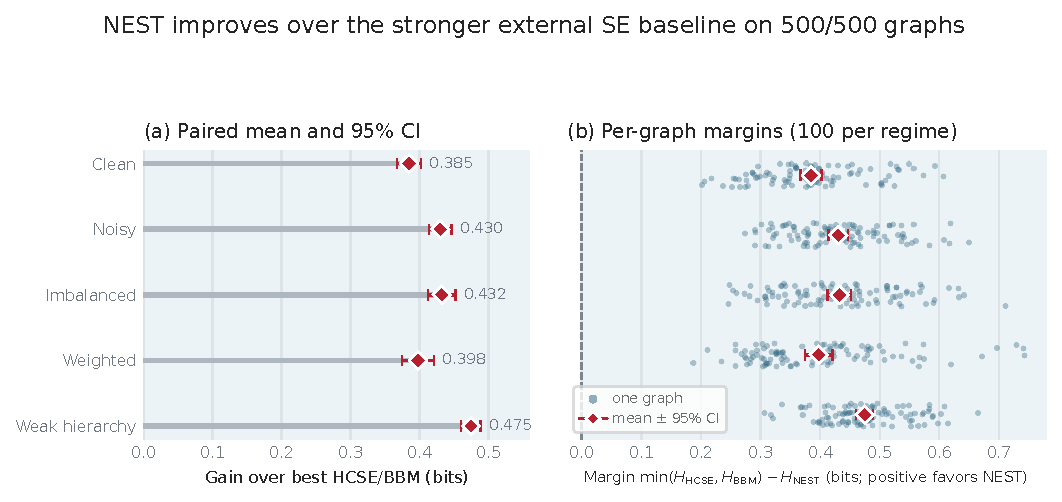
\includegraphics[width=\textwidth]{benchmark_entropy.pdf}
\caption{Rotation-only \NEST against the stronger of HCSE and BBM on each
graph. A positive margin means that \NEST has lower structural entropy. The
left panel reports regime means and paired 95\% confidence intervals. In the
right panel, each blue point is one graph, red diamonds are regime means, and
horizontal whiskers are their paired 95\% confidence intervals.}
\label{fig:entropy-journal}
\end{figure}

\subsection{Frozen exact-optimum audit}

After disjoint calibration fixed 32 candidates per method, the exact audit
sealed 250 graphs at $n=12$, 100 at $n=14$, and 25 at $n=16$. The exact subset
dynamic program is used only for evaluation. Table~\ref{tab:exact-scale}
reports the rotation-only results that produced the five diagnostic cases
above.

\begingroup
\setlength{\tabcolsep}{3pt}
\begin{table}[H]
\centering\small
\caption{Sealed exact-optimum audit on independently generated HSBMs with $n$
vertices and 32 candidates per method: coalescent starts for \NEST, target
heights for HCSE, and label-free cluster counts for BBM. Exact columns report
optimum hits over the listed graphs. The \NEST interval is an exact 95\% Clopper--Pearson
interval for its hit rate. Its relative gap is
$100(H^T_{\mathrm{NEST}}-H^*)/H^*$, reported as mean/worst; zero is optimal.
Candidate selection does not use $H^*$.}
\label{tab:exact-scale}
\begin{tabular*}{\textwidth}{@{\extracolsep{\fill}}rrccccc@{}}
\toprule
& & \multicolumn{3}{c}{Exact optima found}
& \multicolumn{2}{c}{\NEST diagnostics} \\
\cmidrule(lr){3-5}\cmidrule(lr){6-7}
$n$ & Graphs & \NEST & HCSE & BBM
& \shortstack{95\% hit-rate\\interval}
& \shortstack{Mean / worst\\relative gap} \\
\midrule
12 & 250 & \textbf{249/250} & 2/250 & 1/250 & [97.79, 99.99]\% & 0.00032\% / 0.07990\% \\
14 & 100 & \textbf{99/100} & 0/100 & 0/100 & [94.55, 99.97]\% & 0.00121\% / 0.12060\% \\
16 & 25 & \textbf{22/25} & 0/25 & 0/25 & [68.78, 97.45]\% & 0.03990\% / 0.44934\% \\
\bottomrule
\end{tabular*}
\end{table}

\endgroup

Rotation-only \NEST reaches 370 of 375 exact optima, compared with 2/375 for
HCSE and 1/375 for label-free BBM under the declared 32-candidate protocol.
The graft audit closes these five observed \NEST gaps. A disjoint confirmatory
protocol has been frozen before execution on graph seeds 500--519 in each of
the five regimes. It keeps the 32-start rotation-only endpoint as a paired
control, adds exhaustive graft refinement without label-based selection, and
computes the exact optimum only after both endpoints have been selected. Its
primary endpoints are the paired exact-hit difference and the paired entropy
change; runtime and candidate counts are secondary endpoints. Results from
that protocol will replace this paragraph only after the frozen artifact
passes integrity checks.

\section{Related work}\label{sec:related}

\paragraph{Structural entropy.}
Structural information was introduced to measure network organization with an
encoding tree~\cite{li2016}. HCSE and BBM construct structural-entropy
hierarchies through partitioning, merging, and balancing operations
\cite{pan2025}. SuperTAD establishes binary sufficiency and develops
contiguity-aware dynamic programs for chromatin hierarchies
\cite{zhang2021supertad}. Our work instead studies the complexity of a balanced
partitioning restriction and exact topology edits in arbitrary weighted graph
hierarchies. The broader theory and applications are reviewed in
\cite{su2025survey}.

\paragraph{Graph hierarchical clustering.}
Paris constructs graph dendrograms through node-pair sampling
\cite{bonald2018paris}, while Louvain optimizes a flat modularity objective
\cite{blondel2008}. Dasgupta's hierarchical cost and the Moseley--Wang revenue
objective have motivated algorithms and approximation analyses
\cite{dasgupta2016,moseley2017}. Their objectives differ from structural
entropy, but they share the principle that an edge contribution depends on a
cluster associated with its endpoints. Section~\ref{sec:discussion} identifies
edge--LCA objectives as the natural domain for extending our edit calculus.

\paragraph{Tree rearrangement.}
NNI is a classical local move in phylogenetic tree space, where even the
distance between two trees is nontrivial~\cite{litrompzhang1996}. Local NNI
search has also been studied for hierarchical-clustering costs
~\cite{jowhari2024}. PERCH uses rotations to preserve purity during online
construction~\cite{kobren2017perch}. GRINCH adds grafting to repair mistakes
that cannot be corrected by local rotations alone~\cite{monath2019grinch}.
Our contribution is an objective-specific exact calculus: both NNI and graft
are scored against weighted graph structural entropy, every accepted endpoint
is independently verified, and exhaustive termination certifies the declared
neighborhood.

\paragraph{Exact hierarchy optimization and graph partitioning.}
Cluster trellises organize exact inference over subset states
\cite{macaluso2021}; our dynamic program specializes this principle to
structural entropy. The hardness argument draws on the established complexity
of graph bisection in regular graphs~\cite{bui1987graph}
and uses an exact affine identity rather than an approximation between
objectives.

\section{Discussion and extensions}\label{sec:discussion}

The results expose a useful division of labor. The balanced-bisection theorem
shows that a hard cut problem is already present in a restricted
two-dimensional objective. The edit theorems then provide exact, auditable
progress within the much larger encoding-tree space. Hardness motivates
certified approximation by search; local certificates state precisely what
that search has exhausted.

Grafting enlarges the neighborhood without changing the objective. One NNI is
a particular graft, while a long-range graft can relocate a subtree across
several levels in one committed step. On the five diagnosed cases,
rotation-only search had reached a one-NNI certificate while the larger graft
neighborhood still contained decreasing moves. The path formula further
indicates how to scale the operation. Cached module volumes, cuts, and affected
LCA buckets can replace full candidate reconstruction, and candidates at a
fixed tree can be scored in parallel on CPU or GPU.

The edge--LCA derivation also suggests a broader objective class. Any objective
of the form
\[
 F_\phi(T;G)=\sum_{uv\in E}w_{uv}\,
 \phi\!\left(V_{\lca_T(u,v)},d_u,d_v;G\right)
\]
admits a graft difference obtained by subtracting the old and new LCA terms.
Whether that difference has a compact path cache depends on the sufficient
statistics used by $\phi$. Dasgupta cost and Moseley--Wang revenue are natural
test cases, but a general theorem should be claimed only after the formulas and
implementations are verified for non-equivalent objectives.

The present evidence has two boundaries. The hardness theorem concerns a
balanced height-two restriction, whereas the search algorithm operates over
unrestricted binary encoding trees. The exact formulas connect these parts
through one objective but do not turn the constrained hardness result into a
hardness theorem for unrestricted tree optimization. In addition, the five
graft repairs are diagnostic cases; the frozen disjoint suite is needed to
estimate how often the larger neighborhood helps beyond those cases.

Three theoretical questions remain especially important. First, transferring
Theorem~\ref{thm:balanced-hardness} to unconstrained two-dimensional or
unrestricted tree structural entropy requires a valid balance-forcing or
normal-form construction. Second, the number and barrier profile of NNIs
needed to simulate a graft should be bounded in terms of source--target tree
distance. Third, restricted graph families may admit polynomial algorithms or
stronger optimality certificates. These questions define the next stage of
the journal analysis rather than changing the proved claims above.

\section{Conclusion}\label{sec:conclusion}

We connected a hard partitioning core with exact optimization geometry for
structural-entropy hierarchies. Balanced two-module optimization is NP-hard on
cubic graphs through an exact equivalence with Minimum Bisection. Within tree
space, exact NNI and graft identities support monotone search and explicit
neighborhood certificates. The graft neighborhood contains every NNI move and
repairs all five diagnosed failures of rotation-only search. Independent
formulas, full recomputation, exact dynamic programming, and frozen manifests
make each layer of evidence separately checkable. The remaining empirical
question is quantified by a disjoint, frozen graft-confirmation protocol;
algorithmic scaling requires replacing the correctness-first full rescoring
with validated path caches and parallel candidate evaluation.


\section*{Data and code availability}
The implementation, deterministic validators, frozen manifests, and raw
per-instance records are maintained in the project repository. Each numerical
claim in this article is generated from a versioned JSON artifact and can be
recomputed by the accompanying verification scripts. A permanent archival
identifier will be added to the accepted version.

\section*{Declaration of generative AI and AI-assisted technologies in the
writing process}
During manuscript preparation, the authors used OpenAI Codex to assist with
manuscript organization, language editing, code review, and mechanical
consistency checks. The authors reviewed and edited all generated material,
independently checked the proofs, references, code, and numerical results, and
take full responsibility for the content of the article.

\bibliographystyle{elsarticle-num}
\bibliography{base_refs,references}

\appendix
\section{Additional derivations and audit details}\label{app:details}

\subsection{Derivation of the partition form}

For a height-two partition, split Eq.~\eqref{eq:tree-se-journal} into leaf and
module terms:
\[
H^{\mathcal P}(G)=
-\frac{1}{M}\sum_ud_u\log_2\frac{d_u}{V_{S(u)}}
-\frac{1}{M}\sum_i g_i\log_2\frac{V_i}{M}.
\]
Expanding the logarithms and collecting the graph-only term gives
\[
C_G+\frac{1}{M}\sum_i[(V_i-g_i)\log_2V_i+g_i\log_2M].
\]
Because $V_i=2e_i+g_i$ in an undirected graph, this is
Eq.~\eqref{eq:partition-form}.

\subsection{Derivation of the edge--LCA expansion}

For one edge $uv$, its weight appears in the cut $g_{S_a}$ precisely when
$S_a$ contains one endpoint but not the other. Along the $u$ side, the
corresponding logarithms telescope from $d_u$ to
$V_{\lca_T(u,v)}$; the $v$ side telescopes analogously. Hence the contribution
of $uv$ is
\[
\frac{w_{uv}}{M}\left[
\log_2\frac{V_{\lca_T(u,v)}}{d_u}+
\log_2\frac{V_{\lca_T(u,v)}}{d_v}\right],
\]
which equals its term in Eq.~\eqref{eq:edge-lca-journal}.

\subsection{Why a source-cut shortcut is insufficient}

It is tempting to evaluate a graft using only edges crossing the relocated
subtree $S$. This is incorrect. An ancestor on the insertion path gains the
volume of $S$, while an ancestor on the removal path loses it. An edge with
both endpoints outside $S$ may have one of these ancestors as its old or new
LCA, and its logarithmic contribution can therefore change. The deterministic
validator contains a counterexample in which the cut-only shortcut predicts
$-0.119611$ bits while full recomputation gives $+0.106521$ bits. The
edge--LCA and changed-incidence formulas both return the latter value.

\subsection{Exact-audit protocol for the five repaired cases}

The five graphs are identified by the frozen $n=12,14,16$ manifests. For each
graph, the diagnostic script reconstructs the original 32 pairwise-coalescent
starts, runs the same NNI and bounded two-step refinement, and verifies the
recorded pre-graft minimum. It then applies exhaustive best-improvement graft
refinement with NNI descent after every accepted graft. Candidate selection is
based only on structural entropy. The exact dynamic-programming value is
queried after selecting the best of the 32 endpoints. The per-restart traces,
accepted graft counts, elapsed times, and before/after objectives are stored in
the accompanying JSON artifact.


\end{document}
